

\section{Performance metrics}
\label{sec:performance-metrics}
\subsection*{Latency}

The delay between packet's transmission from one node to another is one of the 
most crucial network performance parameters. Although IEEE 802.15.4 networks are not
designed for high data rates, the latency is a valuable metric which depends on a variety of 
factors.

The latency is computed as a half of Round Trip Time (RTT)- the full delay between sending the packet from one node and receiving it from the destination node. Figure \ref{fig:round_trip}  depicts the round trip of a packet.
\vspace{2em}

\begin{figure} [H]
    \centering
    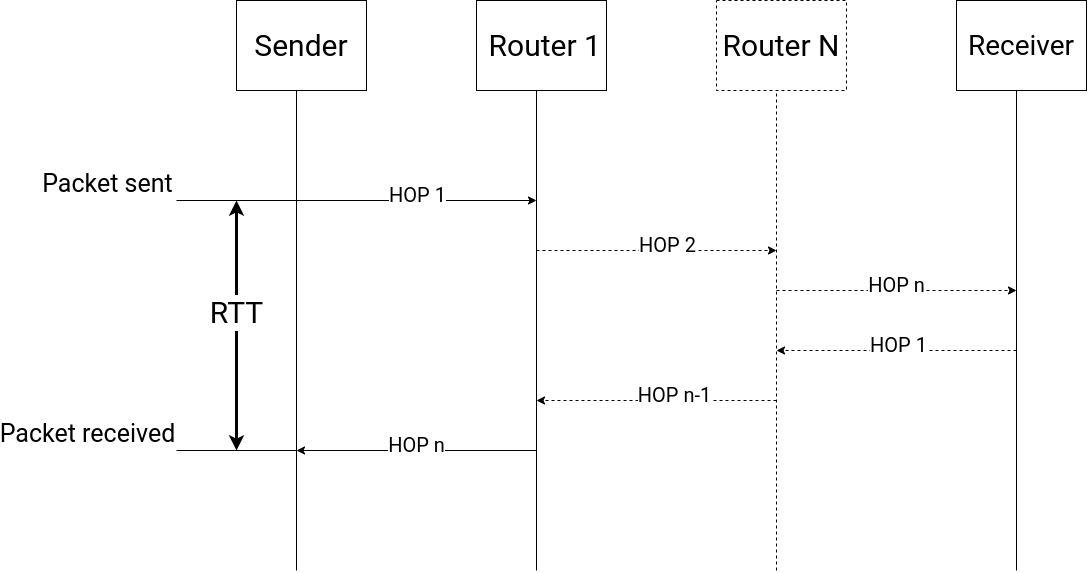
\includegraphics[scale=0.3]{images/rtt-diagram.png}
    \caption{A packet's round trip}
    \label{fig:round_trip}
\end{figure}

In this thesis, RTT was determined by dedicated applications running on a nodes in the
network (either Zigbee or Thread). Additionally, the RTT was selectively 
calculated using packets timestamps from traffic dump collected with Wireshark (sec. 
\ref{sec:benchmark}). However, the latter was used rarely and mainly for ensuring the
calculations correctness performed by applications. These are described in 
details in sections \ref{sec:benchmark} and \ref{sec:zperf}.

One of aspects, which latency depends most on, is the network topology. In this thesis,
the latency was measures in the relationship to the number of hops the packet must go through 
from the sender node to the destination.

Another factor affecting the time of packet delivery is length of sent payload data. 
Experiments performed for this thesis used different lengths of data- from 0 to 79 bytes. This parameter has a direct impact on the packet's 
time in the air. At this point, sending an empty payload (which length equals to 0 
bytes) can seemingly be pointless. However, term \textbf{payload length} refers to the
length of data sent through an application layer and shouldn't be confused with a IEEE 802.15.4 
payload. That said, a packet carrying an empty payload can be valuable as well. An 
exemplary use case for such a packet is sending a notification utilizing only an 
application layer header without any payload.


\subsection*{Throughput}

The overall effective data transmission rate is referred as \textbf{throughput} and expressed in kilobits per second (\textbf{kbps}). In this project, throughput was calculated as a ratio of successfully exchanged data between the sender and received and the overall time of a single experiment. Each run of the experiment
was approximately 10 seconds long and about 150 packets were transmitted from the sender. Figure \ref{fig:throughput} depicts the methodology of throughput calculation.

\begin{figure}[H]
    \centering
    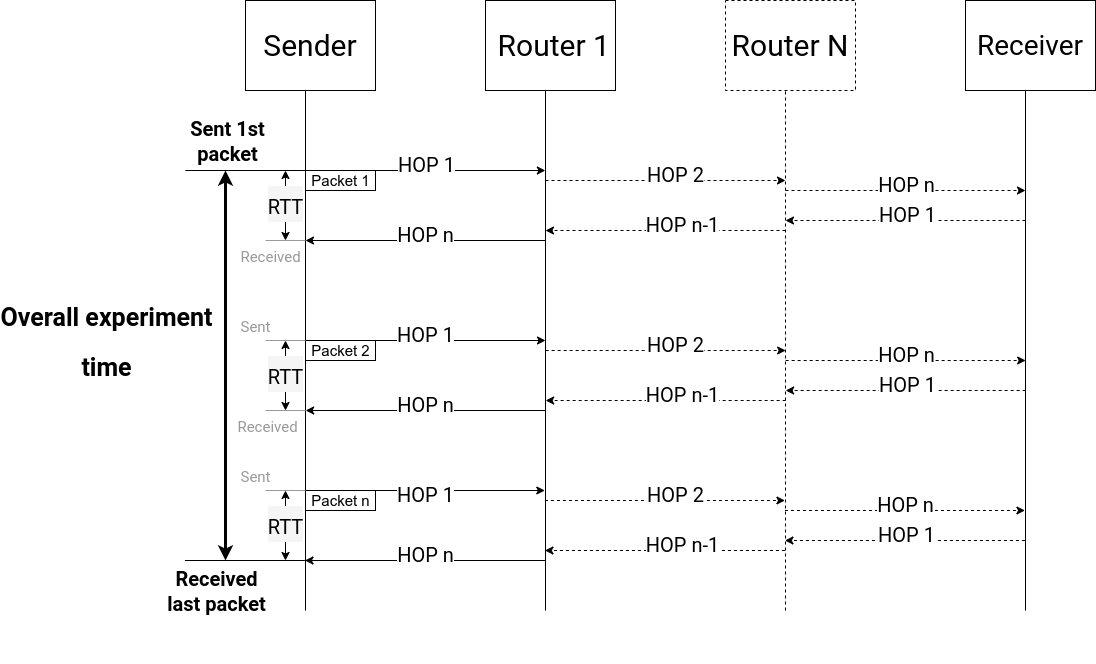
\includegraphics[scale=0.35]{images/throughput-diagram.drawio.png}
    \caption{An overall experiment time calculation.}
    \label{fig:throughput}
\end{figure}

\section{Tools used for testing}

\medskip


\subsection{Hardware}
 The platform chosen for test implementation was Nordic Semiconductor nRF52840. This SoC features 2.4 GHz 
 radio and supports a broad variety of wireless protocols. Except for the bare Soc intended to assembly in a 
 custom PCB, the device is manufactured in two main versions: nRF52840 DK and nRF52840 Dongle. Both of them were 
 utilized for this thesis.
 
 Mesh networks were deployed onto the set of 7 nrf52840 DK boards shown in the figure \ref{fig:test_boards}. All devices were connected to the
 workstation via USB cables.

\begin{figure}[H]
    \centering
    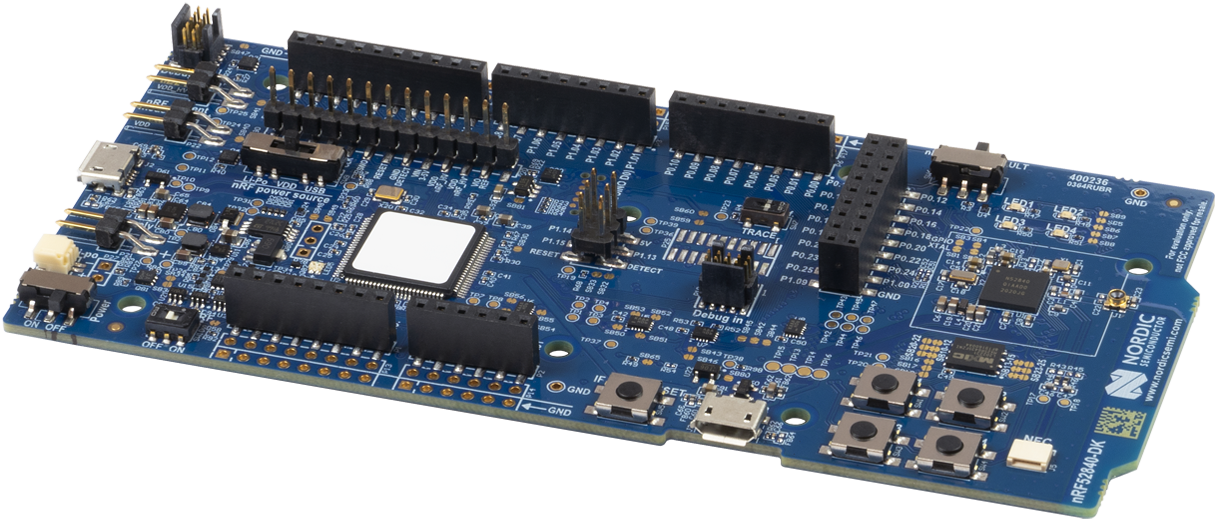
\includegraphics[scale=0.3]{images/test_boards.png}
    \caption{The nRF52840 DK, from nordicsemi.com.}
    \label{fig:test_boards}
\end{figure}

\subsection{Benchmark application}
\label{sec:benchmark}

The most recent implementation of Zigbee and Thread protocols for nRF52840 are shipped as a components of nRF
Connect  SDK (abbreviated as \textbf{NCS}). The SDK does not feature any tool which can be used for 
benchmarking Thread and Zigbee. However, such an application existed before- in the previous Nordic Semiconductor SDK (nRF5 SDK for Thread and Zigbee) and was called \textbf{benchmark}. When implementing tests, the tool based on 
it was implemented and used to perform tests of a Zigbee network.

\subsection*{Benchmark implementation details}


\subsection{Zperf application}
\label{sec:zperf}

Since Thread protocol is an Internet oriented protocol, an existing methodologies and tools could have possibly been used to measure network performance. \textbf{Iperf} is one of the tools created for evaluating performance metrics. A sample application implementing Iperf's API is available in Zephyr RTOS and is called \textbf{Zperf}. For this project, the RTT measurement for UDP based connections and support for Thread was added to the \textbf{Zperf} application.

\subsection*{Zperf implementation details}

\subsection{Other tools used for diagnostics}
\label{sec:tools}

The exploration of computer networks is usually done by eavesdropping the network link between entities. That kind of capturing packets is called \textbf{sniffing} and can be done by a special software. In this case, the traffic of Zigbee and Thread networks was sniffed by \textbf{Wireshark}. 

Any software is not able to operate without a hardware. When IP networks are diagnosed, a network 
interface card (either wired or wireless) available in any modern computer is utilized. Unfortunately, 
sniffing IEEE 802.15.4 requires special network interface. In this thesis, nRF52840 Dongle flashed with 
a dedicated firmware was used.

\medskip
\section{Test setup}
\subsection{Network topology}
\label{sec:network-topology}

As mentioned in the section \ref{sec:performance-metrics}, both of the measures metrics are affected by
the network topology. If the trip of the packet is followed, it is not surprising that the time of its 
delivery between nodes is strictly bonded with the number of hops. The mesh networks routing is designed to deliver packets using the most efficient path. Although the routing algorithm differs between Zigbee and Thread,
the general principle is similar. Routers choose the path to relay packets in such a way, the \textbf{cost}
of the packets delivery is as small as possible \cite{TexasZigbeeVsThread}. That way of forming a network topology
was one of the obstacles encountered during preparation for this project. An explanation and more detailed
description can be found in section \ref{sec:problems-encountered}.

The measurement of latency and throughput in reference to the number of hops requires the network topology
to provide a deterministic number of hops between given nodes. It was decided to test the network performance
against 1 to 6 hops. That need could be met only by introducing a network topology similar to \textbf{daisy 
chain} where any node can have only 1 or 2 connections to the other nodes. Figure \ref{fig:daisy_chain} 
presents the general idea of such a topology.

\medskip
\begin{figure}[H]
    \centering
    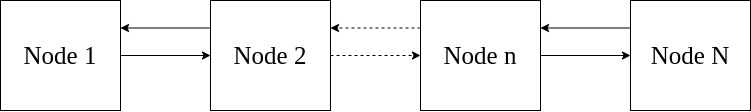
\includegraphics[scale=0.6]{images/daisy-chain.png}
    \caption{The daisy chain topology.}
    \label{fig:daisy_chain}
\end{figure}

It is worth to mention that introduced topology is neither optimal nor energy 
efficient for the devices in the network. Although, it's really hard to 
establish a mesh network that would allow to measure performance in the relation
to the number of hops. 

Setting up a mesh network that would use the topology described above was one
of the problems encountered during the test preparation and has been broadly
described in section \ref{sec:problems-encountered}.

\medskip
\section{Problems encountered}
\label{sec:problems-encountered}

While developing the test methodology, especially the part consisting of
setting up the network (\ref{sec:network-topology}), a number of problems 
arose. A number of ways of solving them had been attempted before a satisfying 
solution was found.

\subsection{Enforcing the network topology}

The
routing in mesh network is based on a cost of given paths, which 
relates to the quality of wireless link between devices. This gives an 
opportunity to build the network topology by tweaking the transmission power
of devices. However, it is rarely possible to do so in practice, because 2.4GHz 
band is broadly used by other electronic goods present around us (for example 
WiFi access points, Bluetooth headphones etc.). Besides the crowded band, 
furnishings and other equipment introduce interference compounding the link
quality. Taking into account all of these factors, it's very hard to determine
the right level of amplification of each device's transceiver suitable to create
a given network topology, and especially the daisy chain.

\subsection*{Using different levels of transmission power}
Setting certain levels of transmission power was the first attempt
to build the network required to conduct the tests. This method seemed to be the
most appropriate for the networks which build their topology on the basis of
the effectiveness of the link between nodes. At the early stage of experiment,
the results were promising. However, as soon as the number of nodes in the 
network raises, the method stopped working as expected. Changing the 
transmitting power works for networks built with up to 4 devices. It becomes
very hard to manage if the number of nodes exceeds that number. That limitations come
from the nature of 2.4 GHz band is sensitive for interference. These are caused by
furniture, the location of radio transceivers and even people moving by. It is hard
to determine an appropriate power level for such a sensitive band.

\subsection*{Rearranging devices}
Once the method of using different power settings of devices failed, the next
idea was developed. The issue with the first attempt is that devices located
in the same room are able to communicate with each other. Even though devices
were located in different areas of the room and their transmission power was
decreased, an unwanted direct links between nodes were established.

It was decided to put devices into separate rooms located on different floors to overcome that problem. It is worth to mention that at this stage of project, only Zigbee 
networks were taken for the tests and a variety of modifications were introduced
into the benchmark application (\ref{sec:benchmark}). An 
established network was managed by the Benchmark commands sent to other nodes
from the device located near the workstation. The devices
were located as shown in the figure \ref{fig:floor_plan} and a number of
tests were conducted using this setup.

\begin{figure}[H]
    \centering
    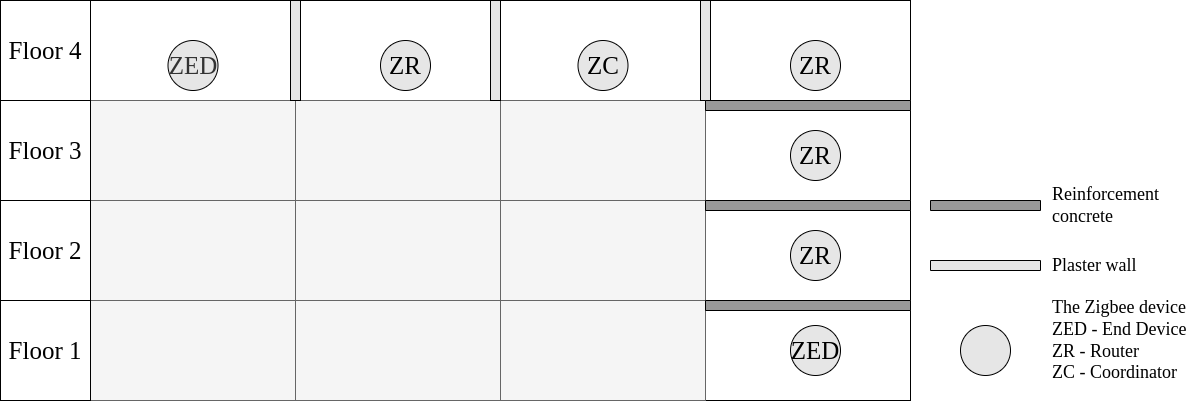
\includegraphics[scale=0.3]{images/floor_plan2.png}
    \caption{The location of devices after rearrangement.}
    \label{fig:floor_plan}
\end{figure}

While having that setup powered on and working for a couple of days, a new 
problem appeared when one node was arbitrarily switched off. A lack of
one router in the network broke an established routing. Although the problematic
device had been switched on back again it was hard to rebuild the old network
topology. This kind of issues enforced a change into the methodology of
creating a network topology to more convenient and easier to manage.

\subsection*{Modifying the software to limit visibility of certain devices}
\label{sec:modifying_visibility}
The described methods and their issues were finally 
worked around using dedicated software configuration of each node. A general 
concept was to limit the visibility of nodes not supposed to exchange data 
with a chosen device.

This method is based on  \textbf{filtering} the devices by their \textbf{IEEE address}.
Zigbee, as well as Thread stack have an API designed especially for this case.
Although long address is not used in every transmitted packet, filtering it
at the stage of associating the device into the network is sufficient to filter
out all unwanted packets.

In case of Zigbee, each device was assigned a long address at a compile time.
A figure \ref{fig:long_address} shows the chosen addressing scheme. Listing 
\ref{lst:zigbee-long-addresses} presents a piece of program where API
for assigning and filtering out addresses is used.  Please note, that
code which  is not not related to setting and filtering the long addresses was cut off the listing.

\begin{figure}[H]
    \centering
    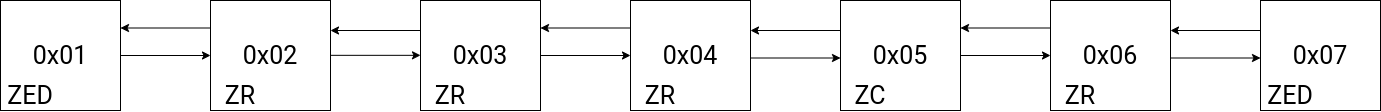
\includegraphics[scale=0.32]{images/zigbee-ieee-address.drawio.png}
    \caption{The Zigbee addressing scheme altogether with devices roles.}
    \label{fig:long_address}
\end{figure}

\begin{lstlisting}[language=C, caption={An usage of the ZBOSS API for assigning and filtering long addresses}, label={lst:zigbee-long-addresses}]
#define DEV_LONG_ADDR                    {0,0,0,0,0,0,0,1}
#define NEIGHBOR1_LONG_ADDR              {0,0,0,0,0,0,0,2}

zb_ieee_addr_t dev_long_addr = DEV_LONG_ADDR;
zb_ieee_addr_t neighbor_long_addr = NEIGHBOR1_LONG_ADDR;

/*  Macros, global variables and static functions declarations */

void main(void) {
    /* Initialization */

    /* Assigning an IEEE address */
    zb_set_long_address(dev_long_addr);

    /* Filtering out all devices except the one with
     * neighbor_long_addr assigned. */
    mac_add_visible_device(neighbor_long_addr);

    /* Enabling the application */
}
\end{lstlisting}

Assigning and filtering out long addresses at a compile time requires to know
them before the firmware is built and flashed onto boards. This was not 
problematic in this case, but it is worth to consider to extend the 
\textit{shell} subsystem with commands for performing these operations at 
run-time.

In case of OpenThread stack, options needed
for long addresses management are built into its CLI subsystem. Addresses 
assignment as well as filtering was done during device's setup by issuing
certain commands. These are presented in the listing \ref{lst:thread-commands} 
and the full process of preparing the network is covered by the section \ref{sec:tests-automation}.

\begin{lstlisting}[language=bash, label={lst:thread-commands}, caption={Shell OpenThread commands for assigning and filtering IEEE addresses}]
uart$: ot extaddr 0000000000000001
uart$: ot macfilter addr allowlist
uart$: ot macfilter addr add 0000000000000002
\end{lstlisting}

Commands issued in the OpenThread shell cause a similar effect to a direct usage
of an API in case of Zigbee.

\section{Thread network setup automation}
\label{sec:tests-automation}

As a matter of Thread network being based on the CLI interface it was 
relatively easy to incorporate an automation in this field. Every step of 
the network setup is covered by a single command issued to the device by the
Python program. Devices are flashed with the same firmware and connected to
the USB hub before the script is run. When the network is up and running,
the nodes are ready to run performance tests, which is done manually.

The Python script was created in relatively generic way enabling to work with
any number of devices. It is based on loading the configuration files
given by a command line parameters. These are then parsed accordingly to a fixed
json schema (listing \ref{lst:json-schema}). It is required to bond a 
configuration file with the board id, which is used by the script to find an 
appropriate serial port to establish a connection with.

\medskip
\begin{lstlisting}[language=Python, label={lst:thread-automation-script}, caption={The main function of a script for Thread network setup}]
def main():
    logging.basicConfig(format="%(levelname)s: %(message)s", level=logging.DEBUG)

    configs = sys.argv[1:]
    thread_devices = []

    for config in configs:
        if ".json" not in config:
            logging.error(f"{config} is not a .json file")
            exit(-1)

    for config in configs:
        thread_devices.append(ThreadDevice(config))

    logging.info(f"Found {len(thread_devices)} Thread device(s)")
    for dev in thread_devices:
        logging.info(f"Setting up {dev}")
        dev.device_setup()

    for dev in thread_devices:
        _ = input(f"Press any key to start {dev.config.board_id} on {dev._find_tty()}")
        dev.network_up()
\end{lstlisting}

\medskip
\begin{lstlisting}[language=Python, label={lst:json-schema}, caption={The json 
schema used to parse boards configuration files.}]
ot_config_schema = {
    "type" : "object",
    "properties" : {
        "board_id" : {"type" : "number"},
        "baudrate" : {"type" : "number"},
        "panid" : {"type" : "string"},
        "factoryreset" : {"type" : "boolean"},
        "channel" :  {"type" : "number"},
        "networkkey" : {"type" : "string"},
        "extaddr" : {"type" : "string"},
        "allowlist" : {
            "type" : "array",
            "items" : {"type": "string"}
        },
        "zperf_role" : {"enum" : ["client", "server"] }
    }
}
\end{lstlisting}

\medskip
\section{Performance evaluation procedure}
\label{sec:performance-testing-scenario}

\subsection{Zigbee evaluation}

The evaluation process begins with setting up the Zigbee network. Devices
used to test are flashed with the firmware modified as described
in \ref{sec:modifying_visibility} to establish a desired topology. Once the 
network is ready, nodes eligible to take part in the test are discovered by
issuing a benchmark command on one of the border devices:
\begin{lstlisting}
uart$: test peer discover
\end{lstlisting}

\noindent As a result of this command, a list of devices shows up (figure \ref{fig:discovered_zigbee_devices}).
\begin{figure}[H]
    \centering
    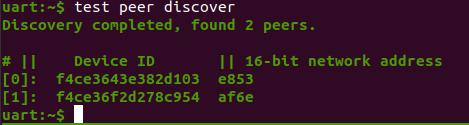
\includegraphics{images/benchmark-devices.jpg}
    \caption{A result of peer discovery command.}
    \label{fig:discovered_zigbee_devices}
\end{figure}

In the next step, a node from the peers listed in \ref{fig:discovered_zigbee_devices} is 
chosen:
\begin{lstlisting}
uart$: test peer select 1
\end{lstlisting}

Then the test configuration is chosen. In the majority of tests executed for the project, tests 
were configured to exchange 150 packets in the mode echo. The length 
of the data was changed in the consecutive tests to cover different cases.
\begin{lstlisting}
uart$: test configure mode echo
uart$: test configure length 64
uart$: test configure count 150
\end{lstlisting}

The final step is to run the test and wait until it finishes.
\begin{lstlisting}
uart$: test start
\end{lstlisting}

The command line remains frozen for the time of test execution. As soon as the test
ends, the results are given and the command line is unblocked. An exemplary test results
are presented in fig. \ref{fig:zigbee_test_results}.
\begin{figure}[H]
    \centering
    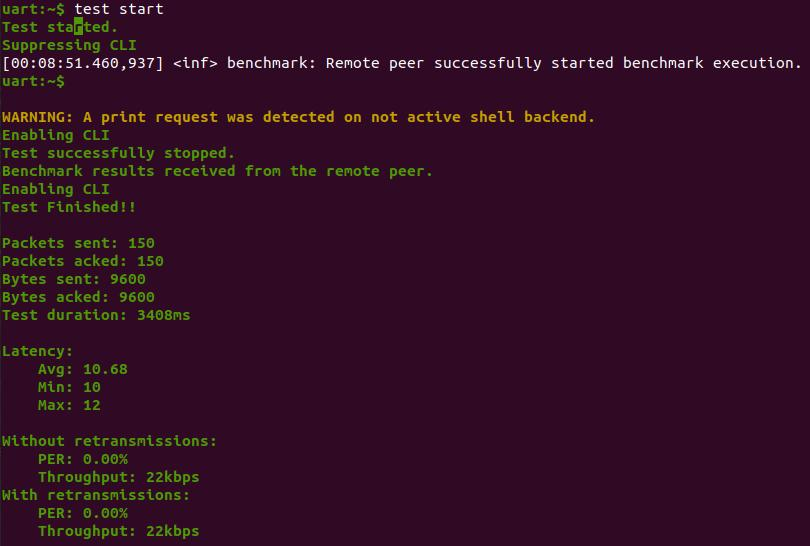
\includegraphics[scale=0.7]{images/zigbee-test-result.jpg}
    \caption{Zigbee benchmark test results.}
    \label{fig:zigbee_test_results}
\end{figure}

\subsection{Thread evaluation}

Thread evaluation process is started with setting up the Thread network as
section \ref{sec:tests-automation} describes. As a next step, the node chosen 
to perform tests with is set up as a zperf server. Zperf needs to be configured 
with an ip address of a node:

\begin{lstlisting}[label={lst:setting_zperf}]
uart$: ot ipaddr
fdde:ad00:beef:0:0:ff:fe00:0
fdde:ad00:beef:0:558:f56b:d688:799
fe80:0:0:0:f3d9:2a82:c8d8:fe43
Done
uart$: zperf setip fdde:ad00:beef:0:558:f56b:d688:799 64
Done
\end{lstlisting}

Then, udp server is started:

\begin{lstlisting}
uart$: zperf udp download 5001 
\end{lstlisting}

Finally, another node is configured with ip address as well and starts 
uploading the data onto the previously configured server node:
\begin{lstlisting}
uart$: ot ipaddr
fdde:ad00:beef:0:0:ff:fe00:0
fdde:ad00:beef:0:558:f56b:d682:795
fe80:0:0:0:f3d9:2a82:c8d8:fe43
Done
uart$: zperf setip fdde:ad00:beef:0:558:f56b:d682:795 64
Done
uart$: zperf udp upload fdde:ad00:beef:0:558:f56b:d688:799 5001 10 50 1M
\end{lstlisting}

The command line is frozen for the time of test execution. At the end of
run, results show up in the output of both devices.

\begin{figure}[H]
    \centering
    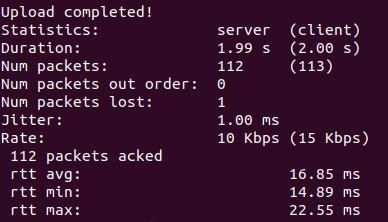
\includegraphics[]{images/zperf-client.jpg}
    \caption{Results on the client side.}
    \label{fig:zperf_client_results}
\end{figure}

\begin{figure}[H]
    \centering
    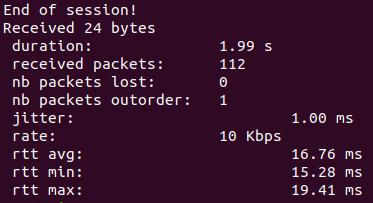
\includegraphics[]{images/zperf-server.jpg}
    \caption{Results on the server side}
    \label{fig:zperf_server_results}
\end{figure}

\medskip
\section{Test results verification}
\label{sec:test-results-verification}

The performance metrics are computed and obtained from the nodes residing inside 
the tested networks. It should not be assumed that the results are legitimate without
analyzing them. The Wireshark program altogether with nRF 802.15.4 Sniffer were used for verification of the gathered results correctness. This method was used mainly during development of testing
software to make sure the algorithm used for calculating the metrics was correct.

\textit{Please note that despite benchmark verification is described in this section, zperf was tested using similar scenario.} The verification test run was executed in the following stages:

\begin{enumerate}
    \itemsep0em
    \item Flash two nRF52840 DKs with benchmark software.
    \item Start recording the network activity with Wireshark and nRF Sniffer.
    \item Establish a Zigbee network consisting of newly flashed devices.
    \item Configure the test run with the following parameters:
    \begin{itemize}
        \itemsep0em
        \item Test mode: Echo
        \item Packets count: 150
        \item Packet length: 64 bytes 
    \end{itemize}
    \item Execute the test.
    \item Compare the outcome calculated by benchmark with the results 
    from Wireshark.
\end{enumerate}

The \ref{fig:verification} figure presents the setup used for the verification 
altogether with annotated network addresses of devices in the Zigbee network.

\begin{figure}[H]
    \centering
    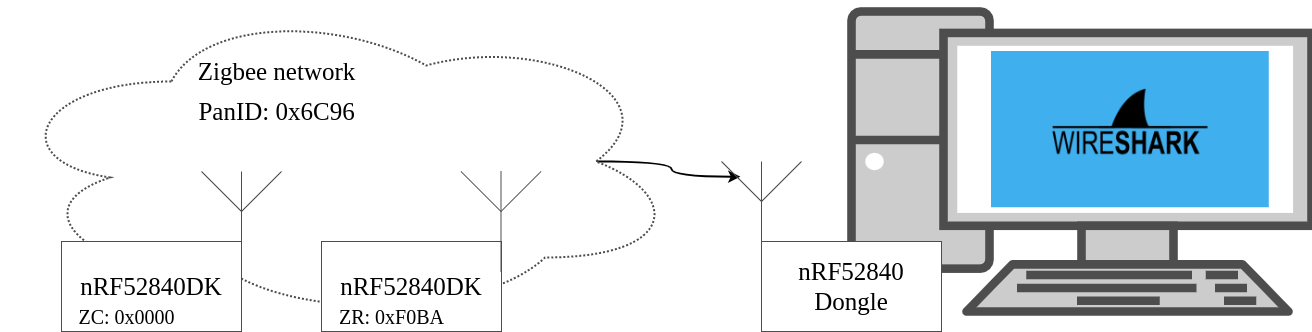
\includegraphics[scale=0.3]{images/verification.png}
    \caption{The network and workstation setup for test results verification.}
    \label{fig:verification}
\end{figure}

When the test finished, benchmark gave results shown in the figure 
\ref{fig:board_results} and the packet stream (shown in the fig. 
\ref{fig:verification_wireshark}) was collected.

\begin{figure}[H]
    \centering
    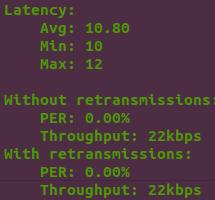
\includegraphics[scale=0.75]{images/one-hop-w-throughput.jpg}
    \caption{The results gathered computed by the benchmark.}
    \label{fig:board_results}
\end{figure}

\begin{figure}[H]
    \centering
    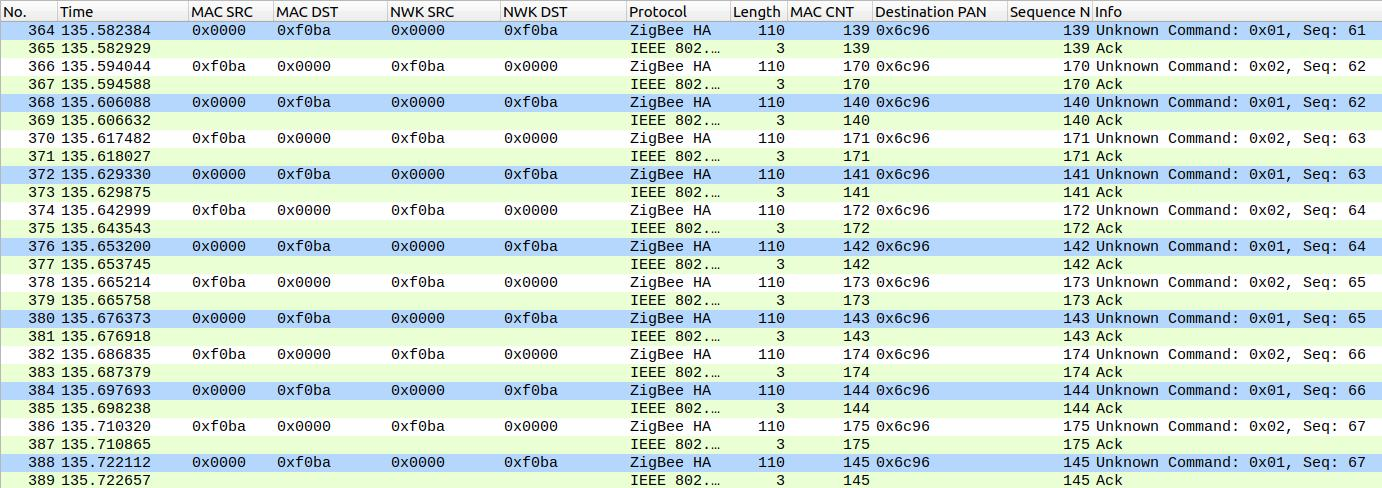
\includegraphics[scale=0.4]{images/packet-stream.jpg}
    \caption{A Wireshark output showing a fragment of the captured packet stream.}
    \label{fig:verification_wireshark}
\end{figure}

A table containing the packets which comes as an output of Wireshark enables
to compute a delay between packets. This is done by using timestamp values
saved in the ``Time'' column. The difference between the transmission 
timestamps of consecutive data packets is interpreted as the latency. 

The packet dump was exported into the .csv file and loaded into a spreadsheet 
for further analysis. Calculated latency measures for this run, alongside with
benchmark results are shown in the table \ref{table:verification}.

\begin{table}[H]
\centering
\begin{tabular}{|c|c|c|c|c|}
\hline
\multirow{2}{*}{Testing tool} & \multicolumn{3}{c|}{Latency} & \multirow{2}{*}{Throughput [kbps]}  \\\cline{2-4}

                  & Average [ms] & Minimum [ms] & Maximum [ms]               &                   \\
\hline
Benchmark & $ 10.80 $  & $ 10.00 $ & $ 12.00 $   &      $22.00$              \\
\hline
Wireshark &  $11.01$ & $10.31$ & $12.76$      &      $22.70$  \\
\hline
\end{tabular}
\caption{A comparison of latency and throughput measurements.}
\label{table:verification}
\end{table}

The results shown differ for all metrics between the benchmark outcome and the 
Wireshark output based calculations. These margins are caused mainly by 
following factors:

\begin{itemize}
    \itemsep0em
    \item The sniffer does not run the network stack which processes the packets before passing them to the application layer. Packets are delivered and marked with a timestamp as soon as they are received.
    \item The sniffer is not located in the exact place as either of tested boards.
    \item The latency in benchmark application is computed as a difference between the time when packet is scheduled to send by the stack and the time
    of response reception. In the method utilizing packets sniffing, the latency
    is expressed as a delay between consecutive packets with data. The difference can come from a time needed by the stack to process the scheduled packet.
\end{itemize}

After summing up above factors, the results yield by the benchmark application
were considered valid and the software was allowed for future use for Zigbee 
performance evaluation. A similar analysis had been conducted for zperf 
application and similar results were obtained. 
